% Created by tikzDevice version 0.7.0 on 2014-10-24 15:37:27
% !TEX encoding = UTF-8 Unicode
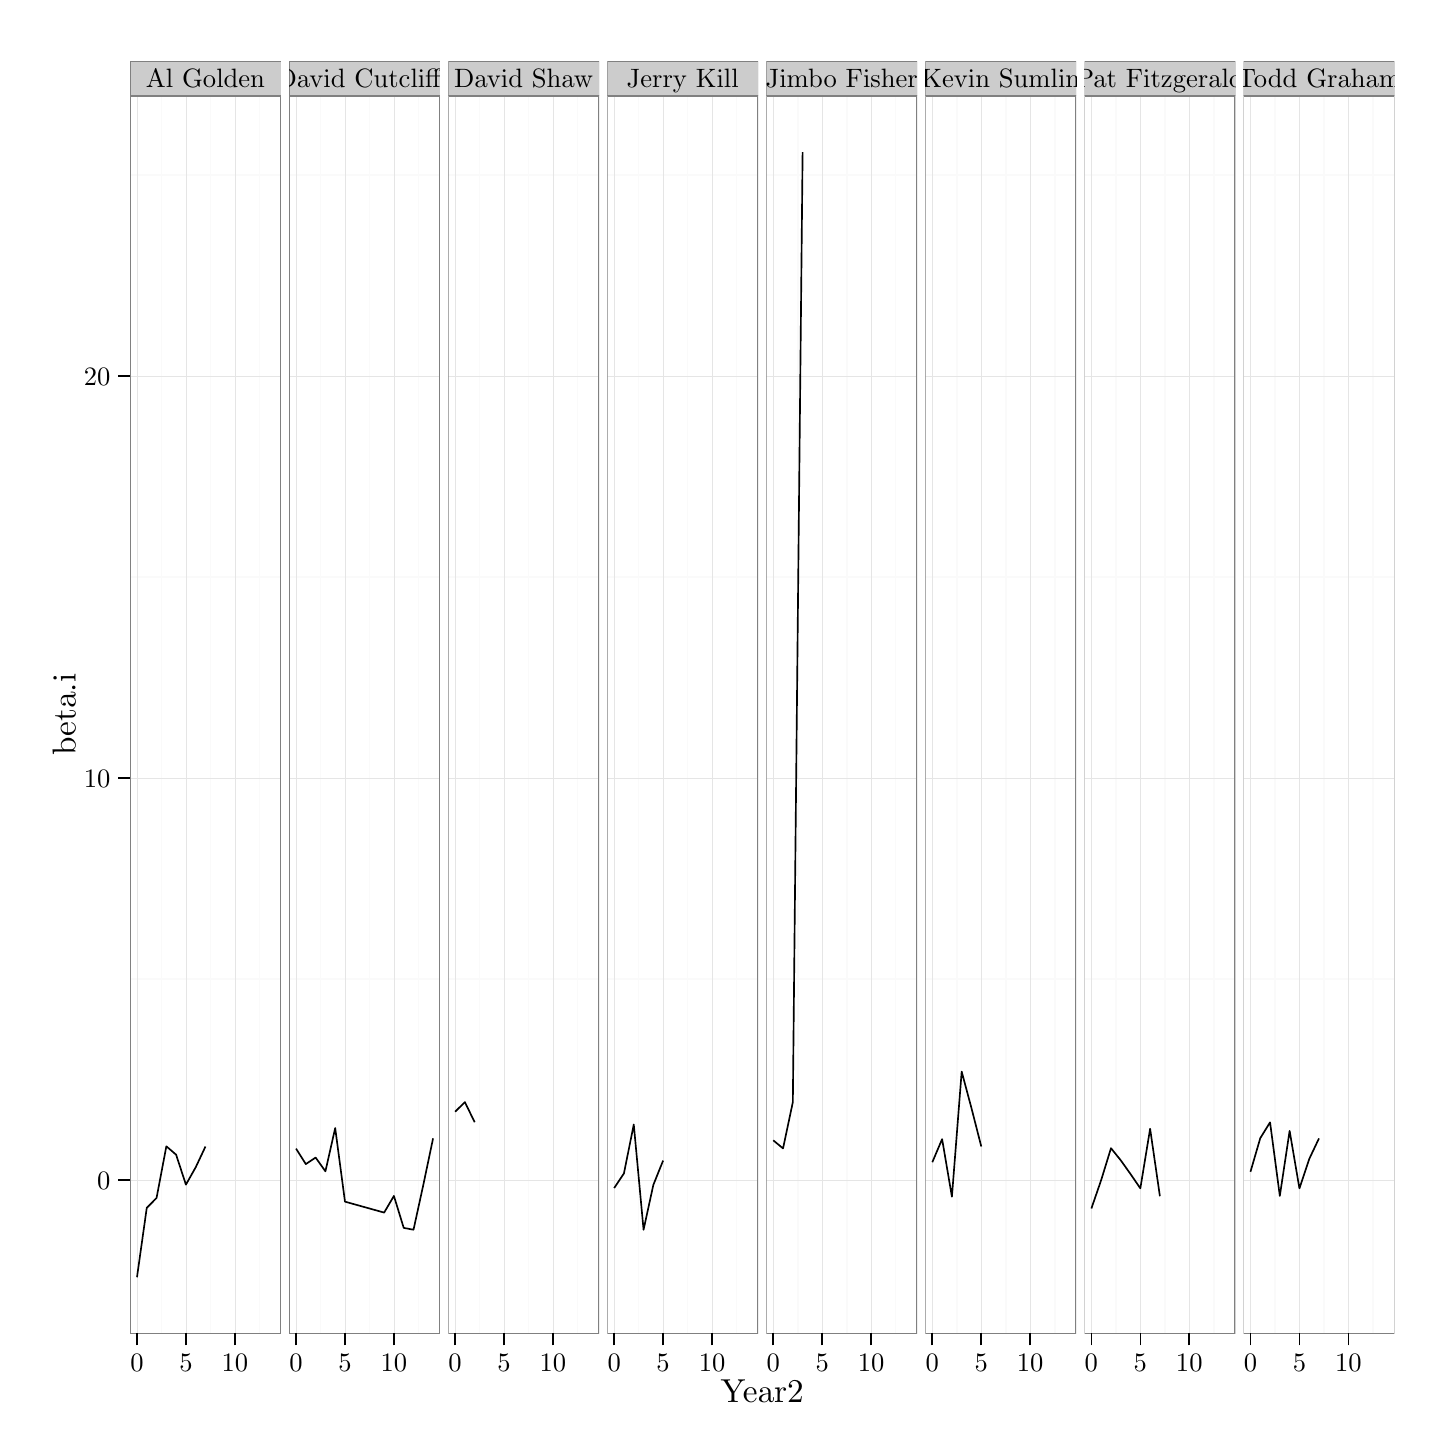
\begin{tikzpicture}[x=1pt,y=1pt]
\definecolor[named]{fillColor}{rgb}{1.00,1.00,1.00}
\path[use as bounding box,fill=fillColor,fill opacity=0.00] (0,0) rectangle (505.89,505.89);
\begin{scope}
\path[clip] (  0.00,  0.00) rectangle (505.89,505.89);
\definecolor[named]{drawColor}{rgb}{1.00,1.00,1.00}
\definecolor[named]{fillColor}{rgb}{1.00,1.00,1.00}

\path[draw=drawColor,line width= 0.6pt,line join=round,line cap=round,fill=fillColor] (  0.00,  0.00) rectangle (505.89,505.89);
\end{scope}
\begin{scope}
\path[clip] ( 37.02,481.21) rectangle ( 91.49,493.85);
\definecolor[named]{drawColor}{rgb}{0.50,0.50,0.50}
\definecolor[named]{fillColor}{rgb}{0.80,0.80,0.80}

\path[draw=drawColor,line width= 0.2pt,line join=round,line cap=round,fill=fillColor] ( 37.02,481.21) rectangle ( 91.49,493.85);
\definecolor[named]{drawColor}{rgb}{0.00,0.00,0.00}

\node[text=drawColor,anchor=base,inner sep=0pt, outer sep=0pt, scale=  0.96] at ( 64.25,484.22) {Al Golden};
\end{scope}
\begin{scope}
\path[clip] ( 94.50,481.21) rectangle (148.97,493.85);
\definecolor[named]{drawColor}{rgb}{0.50,0.50,0.50}
\definecolor[named]{fillColor}{rgb}{0.80,0.80,0.80}

\path[draw=drawColor,line width= 0.2pt,line join=round,line cap=round,fill=fillColor] ( 94.50,481.21) rectangle (148.97,493.85);
\definecolor[named]{drawColor}{rgb}{0.00,0.00,0.00}

\node[text=drawColor,anchor=base,inner sep=0pt, outer sep=0pt, scale=  0.96] at (121.73,484.22) {David Cutcliffe};
\end{scope}
\begin{scope}
\path[clip] (151.98,481.21) rectangle (206.45,493.85);
\definecolor[named]{drawColor}{rgb}{0.50,0.50,0.50}
\definecolor[named]{fillColor}{rgb}{0.80,0.80,0.80}

\path[draw=drawColor,line width= 0.2pt,line join=round,line cap=round,fill=fillColor] (151.98,481.21) rectangle (206.45,493.85);
\definecolor[named]{drawColor}{rgb}{0.00,0.00,0.00}

\node[text=drawColor,anchor=base,inner sep=0pt, outer sep=0pt, scale=  0.96] at (179.21,484.22) {David Shaw};
\end{scope}
\begin{scope}
\path[clip] (209.46,481.21) rectangle (263.93,493.85);
\definecolor[named]{drawColor}{rgb}{0.50,0.50,0.50}
\definecolor[named]{fillColor}{rgb}{0.80,0.80,0.80}

\path[draw=drawColor,line width= 0.2pt,line join=round,line cap=round,fill=fillColor] (209.46,481.21) rectangle (263.93,493.85);
\definecolor[named]{drawColor}{rgb}{0.00,0.00,0.00}

\node[text=drawColor,anchor=base,inner sep=0pt, outer sep=0pt, scale=  0.96] at (236.69,484.22) {Jerry Kill};
\end{scope}
\begin{scope}
\path[clip] (266.94,481.21) rectangle (321.41,493.85);
\definecolor[named]{drawColor}{rgb}{0.50,0.50,0.50}
\definecolor[named]{fillColor}{rgb}{0.80,0.80,0.80}

\path[draw=drawColor,line width= 0.2pt,line join=round,line cap=round,fill=fillColor] (266.94,481.21) rectangle (321.41,493.85);
\definecolor[named]{drawColor}{rgb}{0.00,0.00,0.00}

\node[text=drawColor,anchor=base,inner sep=0pt, outer sep=0pt, scale=  0.96] at (294.17,484.22) {Jimbo Fisher};
\end{scope}
\begin{scope}
\path[clip] (324.42,481.21) rectangle (378.89,493.85);
\definecolor[named]{drawColor}{rgb}{0.50,0.50,0.50}
\definecolor[named]{fillColor}{rgb}{0.80,0.80,0.80}

\path[draw=drawColor,line width= 0.2pt,line join=round,line cap=round,fill=fillColor] (324.42,481.21) rectangle (378.89,493.85);
\definecolor[named]{drawColor}{rgb}{0.00,0.00,0.00}

\node[text=drawColor,anchor=base,inner sep=0pt, outer sep=0pt, scale=  0.96] at (351.65,484.22) {Kevin Sumlin};
\end{scope}
\begin{scope}
\path[clip] (381.90,481.21) rectangle (436.37,493.85);
\definecolor[named]{drawColor}{rgb}{0.50,0.50,0.50}
\definecolor[named]{fillColor}{rgb}{0.80,0.80,0.80}

\path[draw=drawColor,line width= 0.2pt,line join=round,line cap=round,fill=fillColor] (381.90,481.21) rectangle (436.37,493.85);
\definecolor[named]{drawColor}{rgb}{0.00,0.00,0.00}

\node[text=drawColor,anchor=base,inner sep=0pt, outer sep=0pt, scale=  0.96] at (409.13,484.22) {Pat Fitzgerald};
\end{scope}
\begin{scope}
\path[clip] (439.38,481.21) rectangle (493.85,493.85);
\definecolor[named]{drawColor}{rgb}{0.50,0.50,0.50}
\definecolor[named]{fillColor}{rgb}{0.80,0.80,0.80}

\path[draw=drawColor,line width= 0.2pt,line join=round,line cap=round,fill=fillColor] (439.38,481.21) rectangle (493.85,493.85);
\definecolor[named]{drawColor}{rgb}{0.00,0.00,0.00}

\node[text=drawColor,anchor=base,inner sep=0pt, outer sep=0pt, scale=  0.96] at (466.61,484.22) {Todd Graham};
\end{scope}
\begin{scope}
\path[clip] ( 37.02, 34.03) rectangle ( 91.49,481.21);
\definecolor[named]{fillColor}{rgb}{1.00,1.00,1.00}

\path[fill=fillColor] ( 37.02, 34.03) rectangle ( 91.49,481.21);
\definecolor[named]{drawColor}{rgb}{0.98,0.98,0.98}

\path[draw=drawColor,line width= 0.6pt,line join=round] ( 37.02,162.16) --
	( 91.49,162.16);

\path[draw=drawColor,line width= 0.6pt,line join=round] ( 37.02,307.41) --
	( 91.49,307.41);

\path[draw=drawColor,line width= 0.6pt,line join=round] ( 37.02,452.66) --
	( 91.49,452.66);

\path[draw=drawColor,line width= 0.6pt,line join=round] ( 48.34, 34.03) --
	( 48.34,481.21);

\path[draw=drawColor,line width= 0.6pt,line join=round] ( 66.02, 34.03) --
	( 66.02,481.21);

\path[draw=drawColor,line width= 0.6pt,line join=round] ( 83.71, 34.03) --
	( 83.71,481.21);
\definecolor[named]{drawColor}{rgb}{0.90,0.90,0.90}

\path[draw=drawColor,line width= 0.2pt,line join=round] ( 37.02, 89.54) --
	( 91.49, 89.54);

\path[draw=drawColor,line width= 0.2pt,line join=round] ( 37.02,234.79) --
	( 91.49,234.79);

\path[draw=drawColor,line width= 0.2pt,line join=round] ( 37.02,380.04) --
	( 91.49,380.04);

\path[draw=drawColor,line width= 0.2pt,line join=round] ( 39.50, 34.03) --
	( 39.50,481.21);

\path[draw=drawColor,line width= 0.2pt,line join=round] ( 57.18, 34.03) --
	( 57.18,481.21);

\path[draw=drawColor,line width= 0.2pt,line join=round] ( 74.87, 34.03) --
	( 74.87,481.21);
\definecolor[named]{drawColor}{rgb}{0.00,0.00,0.00}

\path[draw=drawColor,line width= 0.6pt,line join=round] ( 39.50, 54.36) --
	( 43.03, 79.41) --
	( 46.57, 83.00) --
	( 50.11,101.67) --
	( 53.64, 98.64) --
	( 57.18, 87.81) --
	( 60.72, 94.10) --
	( 64.25,101.60);
\definecolor[named]{drawColor}{rgb}{0.50,0.50,0.50}

\path[draw=drawColor,line width= 0.6pt,line join=round,line cap=round] ( 37.02, 34.03) rectangle ( 91.49,481.21);
\end{scope}
\begin{scope}
\path[clip] ( 94.50, 34.03) rectangle (148.97,481.21);
\definecolor[named]{fillColor}{rgb}{1.00,1.00,1.00}

\path[fill=fillColor] ( 94.50, 34.03) rectangle (148.97,481.21);
\definecolor[named]{drawColor}{rgb}{0.98,0.98,0.98}

\path[draw=drawColor,line width= 0.6pt,line join=round] ( 94.50,162.16) --
	(148.97,162.16);

\path[draw=drawColor,line width= 0.6pt,line join=round] ( 94.50,307.41) --
	(148.97,307.41);

\path[draw=drawColor,line width= 0.6pt,line join=round] ( 94.50,452.66) --
	(148.97,452.66);

\path[draw=drawColor,line width= 0.6pt,line join=round] (105.82, 34.03) --
	(105.82,481.21);

\path[draw=drawColor,line width= 0.6pt,line join=round] (123.50, 34.03) --
	(123.50,481.21);

\path[draw=drawColor,line width= 0.6pt,line join=round] (141.19, 34.03) --
	(141.19,481.21);
\definecolor[named]{drawColor}{rgb}{0.90,0.90,0.90}

\path[draw=drawColor,line width= 0.2pt,line join=round] ( 94.50, 89.54) --
	(148.97, 89.54);

\path[draw=drawColor,line width= 0.2pt,line join=round] ( 94.50,234.79) --
	(148.97,234.79);

\path[draw=drawColor,line width= 0.2pt,line join=round] ( 94.50,380.04) --
	(148.97,380.04);

\path[draw=drawColor,line width= 0.2pt,line join=round] ( 96.98, 34.03) --
	( 96.98,481.21);

\path[draw=drawColor,line width= 0.2pt,line join=round] (114.66, 34.03) --
	(114.66,481.21);

\path[draw=drawColor,line width= 0.2pt,line join=round] (132.34, 34.03) --
	(132.34,481.21);
\definecolor[named]{drawColor}{rgb}{0.00,0.00,0.00}

\path[draw=drawColor,line width= 0.6pt,line join=round] ( 96.98,100.83) --
	(100.51, 95.24) --
	(104.05, 97.60) --
	(107.59, 92.63) --
	(111.12,108.26) --
	(114.66, 81.67) --
	(128.81, 77.72) --
	(132.34, 83.74) --
	(135.88, 72.20) --
	(139.42, 71.52) --
	(142.96, 87.72) --
	(146.49,104.54);
\definecolor[named]{drawColor}{rgb}{0.50,0.50,0.50}

\path[draw=drawColor,line width= 0.6pt,line join=round,line cap=round] ( 94.50, 34.03) rectangle (148.97,481.21);
\end{scope}
\begin{scope}
\path[clip] (151.98, 34.03) rectangle (206.45,481.21);
\definecolor[named]{fillColor}{rgb}{1.00,1.00,1.00}

\path[fill=fillColor] (151.98, 34.03) rectangle (206.45,481.21);
\definecolor[named]{drawColor}{rgb}{0.98,0.98,0.98}

\path[draw=drawColor,line width= 0.6pt,line join=round] (151.98,162.16) --
	(206.45,162.16);

\path[draw=drawColor,line width= 0.6pt,line join=round] (151.98,307.41) --
	(206.45,307.41);

\path[draw=drawColor,line width= 0.6pt,line join=round] (151.98,452.66) --
	(206.45,452.66);

\path[draw=drawColor,line width= 0.6pt,line join=round] (163.30, 34.03) --
	(163.30,481.21);

\path[draw=drawColor,line width= 0.6pt,line join=round] (180.98, 34.03) --
	(180.98,481.21);

\path[draw=drawColor,line width= 0.6pt,line join=round] (198.67, 34.03) --
	(198.67,481.21);
\definecolor[named]{drawColor}{rgb}{0.90,0.90,0.90}

\path[draw=drawColor,line width= 0.2pt,line join=round] (151.98, 89.54) --
	(206.45, 89.54);

\path[draw=drawColor,line width= 0.2pt,line join=round] (151.98,234.79) --
	(206.45,234.79);

\path[draw=drawColor,line width= 0.2pt,line join=round] (151.98,380.04) --
	(206.45,380.04);

\path[draw=drawColor,line width= 0.2pt,line join=round] (154.46, 34.03) --
	(154.46,481.21);

\path[draw=drawColor,line width= 0.2pt,line join=round] (172.14, 34.03) --
	(172.14,481.21);

\path[draw=drawColor,line width= 0.2pt,line join=round] (189.82, 34.03) --
	(189.82,481.21);
\definecolor[named]{drawColor}{rgb}{0.00,0.00,0.00}

\path[draw=drawColor,line width= 0.6pt,line join=round] (154.46,114.18) --
	(157.99,117.63) --
	(161.53,110.36);
\definecolor[named]{drawColor}{rgb}{0.50,0.50,0.50}

\path[draw=drawColor,line width= 0.6pt,line join=round,line cap=round] (151.98, 34.03) rectangle (206.45,481.21);
\end{scope}
\begin{scope}
\path[clip] (209.46, 34.03) rectangle (263.93,481.21);
\definecolor[named]{fillColor}{rgb}{1.00,1.00,1.00}

\path[fill=fillColor] (209.46, 34.03) rectangle (263.93,481.21);
\definecolor[named]{drawColor}{rgb}{0.98,0.98,0.98}

\path[draw=drawColor,line width= 0.6pt,line join=round] (209.46,162.16) --
	(263.93,162.16);

\path[draw=drawColor,line width= 0.6pt,line join=round] (209.46,307.41) --
	(263.93,307.41);

\path[draw=drawColor,line width= 0.6pt,line join=round] (209.46,452.66) --
	(263.93,452.66);

\path[draw=drawColor,line width= 0.6pt,line join=round] (220.78, 34.03) --
	(220.78,481.21);

\path[draw=drawColor,line width= 0.6pt,line join=round] (238.46, 34.03) --
	(238.46,481.21);

\path[draw=drawColor,line width= 0.6pt,line join=round] (256.15, 34.03) --
	(256.15,481.21);
\definecolor[named]{drawColor}{rgb}{0.90,0.90,0.90}

\path[draw=drawColor,line width= 0.2pt,line join=round] (209.46, 89.54) --
	(263.93, 89.54);

\path[draw=drawColor,line width= 0.2pt,line join=round] (209.46,234.79) --
	(263.93,234.79);

\path[draw=drawColor,line width= 0.2pt,line join=round] (209.46,380.04) --
	(263.93,380.04);

\path[draw=drawColor,line width= 0.2pt,line join=round] (211.93, 34.03) --
	(211.93,481.21);

\path[draw=drawColor,line width= 0.2pt,line join=round] (229.62, 34.03) --
	(229.62,481.21);

\path[draw=drawColor,line width= 0.2pt,line join=round] (247.30, 34.03) --
	(247.30,481.21);
\definecolor[named]{drawColor}{rgb}{0.00,0.00,0.00}

\path[draw=drawColor,line width= 0.6pt,line join=round] (211.93, 86.59) --
	(215.47, 91.91) --
	(219.01,109.57) --
	(222.55, 71.52) --
	(226.08, 87.72) --
	(229.62, 96.52);
\definecolor[named]{drawColor}{rgb}{0.50,0.50,0.50}

\path[draw=drawColor,line width= 0.6pt,line join=round,line cap=round] (209.46, 34.03) rectangle (263.93,481.21);
\end{scope}
\begin{scope}
\path[clip] (266.94, 34.03) rectangle (321.41,481.21);
\definecolor[named]{fillColor}{rgb}{1.00,1.00,1.00}

\path[fill=fillColor] (266.94, 34.03) rectangle (321.41,481.21);
\definecolor[named]{drawColor}{rgb}{0.98,0.98,0.98}

\path[draw=drawColor,line width= 0.6pt,line join=round] (266.94,162.16) --
	(321.41,162.16);

\path[draw=drawColor,line width= 0.6pt,line join=round] (266.94,307.41) --
	(321.41,307.41);

\path[draw=drawColor,line width= 0.6pt,line join=round] (266.94,452.66) --
	(321.41,452.66);

\path[draw=drawColor,line width= 0.6pt,line join=round] (278.26, 34.03) --
	(278.26,481.21);

\path[draw=drawColor,line width= 0.6pt,line join=round] (295.94, 34.03) --
	(295.94,481.21);

\path[draw=drawColor,line width= 0.6pt,line join=round] (313.63, 34.03) --
	(313.63,481.21);
\definecolor[named]{drawColor}{rgb}{0.90,0.90,0.90}

\path[draw=drawColor,line width= 0.2pt,line join=round] (266.94, 89.54) --
	(321.41, 89.54);

\path[draw=drawColor,line width= 0.2pt,line join=round] (266.94,234.79) --
	(321.41,234.79);

\path[draw=drawColor,line width= 0.2pt,line join=round] (266.94,380.04) --
	(321.41,380.04);

\path[draw=drawColor,line width= 0.2pt,line join=round] (269.41, 34.03) --
	(269.41,481.21);

\path[draw=drawColor,line width= 0.2pt,line join=round] (287.10, 34.03) --
	(287.10,481.21);

\path[draw=drawColor,line width= 0.2pt,line join=round] (304.78, 34.03) --
	(304.78,481.21);
\definecolor[named]{drawColor}{rgb}{0.00,0.00,0.00}

\path[draw=drawColor,line width= 0.6pt,line join=round] (269.41,103.83) --
	(272.95,100.91) --
	(276.49,117.63) --
	(280.02,460.88);
\definecolor[named]{drawColor}{rgb}{0.50,0.50,0.50}

\path[draw=drawColor,line width= 0.6pt,line join=round,line cap=round] (266.94, 34.03) rectangle (321.41,481.21);
\end{scope}
\begin{scope}
\path[clip] (324.42, 34.03) rectangle (378.89,481.21);
\definecolor[named]{fillColor}{rgb}{1.00,1.00,1.00}

\path[fill=fillColor] (324.42, 34.03) rectangle (378.89,481.21);
\definecolor[named]{drawColor}{rgb}{0.98,0.98,0.98}

\path[draw=drawColor,line width= 0.6pt,line join=round] (324.42,162.16) --
	(378.89,162.16);

\path[draw=drawColor,line width= 0.6pt,line join=round] (324.42,307.41) --
	(378.89,307.41);

\path[draw=drawColor,line width= 0.6pt,line join=round] (324.42,452.66) --
	(378.89,452.66);

\path[draw=drawColor,line width= 0.6pt,line join=round] (335.74, 34.03) --
	(335.74,481.21);

\path[draw=drawColor,line width= 0.6pt,line join=round] (353.42, 34.03) --
	(353.42,481.21);

\path[draw=drawColor,line width= 0.6pt,line join=round] (371.10, 34.03) --
	(371.10,481.21);
\definecolor[named]{drawColor}{rgb}{0.90,0.90,0.90}

\path[draw=drawColor,line width= 0.2pt,line join=round] (324.42, 89.54) --
	(378.89, 89.54);

\path[draw=drawColor,line width= 0.2pt,line join=round] (324.42,234.79) --
	(378.89,234.79);

\path[draw=drawColor,line width= 0.2pt,line join=round] (324.42,380.04) --
	(378.89,380.04);

\path[draw=drawColor,line width= 0.2pt,line join=round] (326.89, 34.03) --
	(326.89,481.21);

\path[draw=drawColor,line width= 0.2pt,line join=round] (344.58, 34.03) --
	(344.58,481.21);

\path[draw=drawColor,line width= 0.2pt,line join=round] (362.26, 34.03) --
	(362.26,481.21);
\definecolor[named]{drawColor}{rgb}{0.00,0.00,0.00}

\path[draw=drawColor,line width= 0.6pt,line join=round] (326.89, 95.92) --
	(330.43,104.28) --
	(333.97, 83.46) --
	(337.50,128.66) --
	(341.04,115.45) --
	(344.58,101.60);
\definecolor[named]{drawColor}{rgb}{0.50,0.50,0.50}

\path[draw=drawColor,line width= 0.6pt,line join=round,line cap=round] (324.42, 34.03) rectangle (378.89,481.21);
\end{scope}
\begin{scope}
\path[clip] (381.90, 34.03) rectangle (436.37,481.21);
\definecolor[named]{fillColor}{rgb}{1.00,1.00,1.00}

\path[fill=fillColor] (381.90, 34.03) rectangle (436.37,481.21);
\definecolor[named]{drawColor}{rgb}{0.98,0.98,0.98}

\path[draw=drawColor,line width= 0.6pt,line join=round] (381.90,162.16) --
	(436.37,162.16);

\path[draw=drawColor,line width= 0.6pt,line join=round] (381.90,307.41) --
	(436.37,307.41);

\path[draw=drawColor,line width= 0.6pt,line join=round] (381.90,452.66) --
	(436.37,452.66);

\path[draw=drawColor,line width= 0.6pt,line join=round] (393.22, 34.03) --
	(393.22,481.21);

\path[draw=drawColor,line width= 0.6pt,line join=round] (410.90, 34.03) --
	(410.90,481.21);

\path[draw=drawColor,line width= 0.6pt,line join=round] (428.58, 34.03) --
	(428.58,481.21);
\definecolor[named]{drawColor}{rgb}{0.90,0.90,0.90}

\path[draw=drawColor,line width= 0.2pt,line join=round] (381.90, 89.54) --
	(436.37, 89.54);

\path[draw=drawColor,line width= 0.2pt,line join=round] (381.90,234.79) --
	(436.37,234.79);

\path[draw=drawColor,line width= 0.2pt,line join=round] (381.90,380.04) --
	(436.37,380.04);

\path[draw=drawColor,line width= 0.2pt,line join=round] (384.37, 34.03) --
	(384.37,481.21);

\path[draw=drawColor,line width= 0.2pt,line join=round] (402.06, 34.03) --
	(402.06,481.21);

\path[draw=drawColor,line width= 0.2pt,line join=round] (419.74, 34.03) --
	(419.74,481.21);
\definecolor[named]{drawColor}{rgb}{0.00,0.00,0.00}

\path[draw=drawColor,line width= 0.6pt,line join=round] (384.37, 79.20) --
	(387.91, 89.49) --
	(391.45,100.99) --
	(394.98, 96.61) --
	(398.52, 91.64) --
	(402.06, 86.47) --
	(405.59,108.01) --
	(409.13, 83.62);
\definecolor[named]{drawColor}{rgb}{0.50,0.50,0.50}

\path[draw=drawColor,line width= 0.6pt,line join=round,line cap=round] (381.90, 34.03) rectangle (436.37,481.21);
\end{scope}
\begin{scope}
\path[clip] (439.38, 34.03) rectangle (493.85,481.21);
\definecolor[named]{fillColor}{rgb}{1.00,1.00,1.00}

\path[fill=fillColor] (439.38, 34.03) rectangle (493.85,481.21);
\definecolor[named]{drawColor}{rgb}{0.98,0.98,0.98}

\path[draw=drawColor,line width= 0.6pt,line join=round] (439.38,162.16) --
	(493.85,162.16);

\path[draw=drawColor,line width= 0.6pt,line join=round] (439.38,307.41) --
	(493.85,307.41);

\path[draw=drawColor,line width= 0.6pt,line join=round] (439.38,452.66) --
	(493.85,452.66);

\path[draw=drawColor,line width= 0.6pt,line join=round] (450.69, 34.03) --
	(450.69,481.21);

\path[draw=drawColor,line width= 0.6pt,line join=round] (468.38, 34.03) --
	(468.38,481.21);

\path[draw=drawColor,line width= 0.6pt,line join=round] (486.06, 34.03) --
	(486.06,481.21);
\definecolor[named]{drawColor}{rgb}{0.90,0.90,0.90}

\path[draw=drawColor,line width= 0.2pt,line join=round] (439.38, 89.54) --
	(493.85, 89.54);

\path[draw=drawColor,line width= 0.2pt,line join=round] (439.38,234.79) --
	(493.85,234.79);

\path[draw=drawColor,line width= 0.2pt,line join=round] (439.38,380.04) --
	(493.85,380.04);

\path[draw=drawColor,line width= 0.2pt,line join=round] (441.85, 34.03) --
	(441.85,481.21);

\path[draw=drawColor,line width= 0.2pt,line join=round] (459.54, 34.03) --
	(459.54,481.21);

\path[draw=drawColor,line width= 0.2pt,line join=round] (477.22, 34.03) --
	(477.22,481.21);
\definecolor[named]{drawColor}{rgb}{0.00,0.00,0.00}

\path[draw=drawColor,line width= 0.6pt,line join=round] (441.85, 92.46) --
	(445.39,104.60) --
	(448.93,110.34) --
	(452.46, 83.74) --
	(456.00,107.26) --
	(459.54, 86.46) --
	(463.07, 97.06) --
	(466.61,104.54);
\definecolor[named]{drawColor}{rgb}{0.50,0.50,0.50}

\path[draw=drawColor,line width= 0.6pt,line join=round,line cap=round] (439.38, 34.03) rectangle (493.85,481.21);
\end{scope}
\begin{scope}
\path[clip] (  0.00,  0.00) rectangle (505.89,505.89);
\definecolor[named]{drawColor}{rgb}{0.00,0.00,0.00}

\node[text=drawColor,anchor=base east,inner sep=0pt, outer sep=0pt, scale=  0.96] at ( 29.91, 86.23) {0};

\node[text=drawColor,anchor=base east,inner sep=0pt, outer sep=0pt, scale=  0.96] at ( 29.91,231.48) {10};

\node[text=drawColor,anchor=base east,inner sep=0pt, outer sep=0pt, scale=  0.96] at ( 29.91,376.73) {20};
\end{scope}
\begin{scope}
\path[clip] (  0.00,  0.00) rectangle (505.89,505.89);
\definecolor[named]{drawColor}{rgb}{0.00,0.00,0.00}

\path[draw=drawColor,line width= 0.6pt,line join=round] ( 32.75, 89.54) --
	( 37.02, 89.54);

\path[draw=drawColor,line width= 0.6pt,line join=round] ( 32.75,234.79) --
	( 37.02,234.79);

\path[draw=drawColor,line width= 0.6pt,line join=round] ( 32.75,380.04) --
	( 37.02,380.04);
\end{scope}
\begin{scope}
\path[clip] (  0.00,  0.00) rectangle (505.89,505.89);
\definecolor[named]{drawColor}{rgb}{0.00,0.00,0.00}

\path[draw=drawColor,line width= 0.6pt,line join=round] ( 39.50, 29.77) --
	( 39.50, 34.03);

\path[draw=drawColor,line width= 0.6pt,line join=round] ( 57.18, 29.77) --
	( 57.18, 34.03);

\path[draw=drawColor,line width= 0.6pt,line join=round] ( 74.87, 29.77) --
	( 74.87, 34.03);
\end{scope}
\begin{scope}
\path[clip] (  0.00,  0.00) rectangle (505.89,505.89);
\definecolor[named]{drawColor}{rgb}{0.00,0.00,0.00}

\node[text=drawColor,anchor=base,inner sep=0pt, outer sep=0pt, scale=  0.96] at ( 39.50, 20.31) {0};

\node[text=drawColor,anchor=base,inner sep=0pt, outer sep=0pt, scale=  0.96] at ( 57.18, 20.31) {5};

\node[text=drawColor,anchor=base,inner sep=0pt, outer sep=0pt, scale=  0.96] at ( 74.87, 20.31) {10};
\end{scope}
\begin{scope}
\path[clip] (  0.00,  0.00) rectangle (505.89,505.89);
\definecolor[named]{drawColor}{rgb}{0.00,0.00,0.00}

\path[draw=drawColor,line width= 0.6pt,line join=round] ( 96.98, 29.77) --
	( 96.98, 34.03);

\path[draw=drawColor,line width= 0.6pt,line join=round] (114.66, 29.77) --
	(114.66, 34.03);

\path[draw=drawColor,line width= 0.6pt,line join=round] (132.34, 29.77) --
	(132.34, 34.03);
\end{scope}
\begin{scope}
\path[clip] (  0.00,  0.00) rectangle (505.89,505.89);
\definecolor[named]{drawColor}{rgb}{0.00,0.00,0.00}

\node[text=drawColor,anchor=base,inner sep=0pt, outer sep=0pt, scale=  0.96] at ( 96.98, 20.31) {0};

\node[text=drawColor,anchor=base,inner sep=0pt, outer sep=0pt, scale=  0.96] at (114.66, 20.31) {5};

\node[text=drawColor,anchor=base,inner sep=0pt, outer sep=0pt, scale=  0.96] at (132.34, 20.31) {10};
\end{scope}
\begin{scope}
\path[clip] (  0.00,  0.00) rectangle (505.89,505.89);
\definecolor[named]{drawColor}{rgb}{0.00,0.00,0.00}

\path[draw=drawColor,line width= 0.6pt,line join=round] (154.46, 29.77) --
	(154.46, 34.03);

\path[draw=drawColor,line width= 0.6pt,line join=round] (172.14, 29.77) --
	(172.14, 34.03);

\path[draw=drawColor,line width= 0.6pt,line join=round] (189.82, 29.77) --
	(189.82, 34.03);
\end{scope}
\begin{scope}
\path[clip] (  0.00,  0.00) rectangle (505.89,505.89);
\definecolor[named]{drawColor}{rgb}{0.00,0.00,0.00}

\node[text=drawColor,anchor=base,inner sep=0pt, outer sep=0pt, scale=  0.96] at (154.46, 20.31) {0};

\node[text=drawColor,anchor=base,inner sep=0pt, outer sep=0pt, scale=  0.96] at (172.14, 20.31) {5};

\node[text=drawColor,anchor=base,inner sep=0pt, outer sep=0pt, scale=  0.96] at (189.82, 20.31) {10};
\end{scope}
\begin{scope}
\path[clip] (  0.00,  0.00) rectangle (505.89,505.89);
\definecolor[named]{drawColor}{rgb}{0.00,0.00,0.00}

\path[draw=drawColor,line width= 0.6pt,line join=round] (211.93, 29.77) --
	(211.93, 34.03);

\path[draw=drawColor,line width= 0.6pt,line join=round] (229.62, 29.77) --
	(229.62, 34.03);

\path[draw=drawColor,line width= 0.6pt,line join=round] (247.30, 29.77) --
	(247.30, 34.03);
\end{scope}
\begin{scope}
\path[clip] (  0.00,  0.00) rectangle (505.89,505.89);
\definecolor[named]{drawColor}{rgb}{0.00,0.00,0.00}

\node[text=drawColor,anchor=base,inner sep=0pt, outer sep=0pt, scale=  0.96] at (211.93, 20.31) {0};

\node[text=drawColor,anchor=base,inner sep=0pt, outer sep=0pt, scale=  0.96] at (229.62, 20.31) {5};

\node[text=drawColor,anchor=base,inner sep=0pt, outer sep=0pt, scale=  0.96] at (247.30, 20.31) {10};
\end{scope}
\begin{scope}
\path[clip] (  0.00,  0.00) rectangle (505.89,505.89);
\definecolor[named]{drawColor}{rgb}{0.00,0.00,0.00}

\path[draw=drawColor,line width= 0.6pt,line join=round] (269.41, 29.77) --
	(269.41, 34.03);

\path[draw=drawColor,line width= 0.6pt,line join=round] (287.10, 29.77) --
	(287.10, 34.03);

\path[draw=drawColor,line width= 0.6pt,line join=round] (304.78, 29.77) --
	(304.78, 34.03);
\end{scope}
\begin{scope}
\path[clip] (  0.00,  0.00) rectangle (505.89,505.89);
\definecolor[named]{drawColor}{rgb}{0.00,0.00,0.00}

\node[text=drawColor,anchor=base,inner sep=0pt, outer sep=0pt, scale=  0.96] at (269.41, 20.31) {0};

\node[text=drawColor,anchor=base,inner sep=0pt, outer sep=0pt, scale=  0.96] at (287.10, 20.31) {5};

\node[text=drawColor,anchor=base,inner sep=0pt, outer sep=0pt, scale=  0.96] at (304.78, 20.31) {10};
\end{scope}
\begin{scope}
\path[clip] (  0.00,  0.00) rectangle (505.89,505.89);
\definecolor[named]{drawColor}{rgb}{0.00,0.00,0.00}

\path[draw=drawColor,line width= 0.6pt,line join=round] (326.89, 29.77) --
	(326.89, 34.03);

\path[draw=drawColor,line width= 0.6pt,line join=round] (344.58, 29.77) --
	(344.58, 34.03);

\path[draw=drawColor,line width= 0.6pt,line join=round] (362.26, 29.77) --
	(362.26, 34.03);
\end{scope}
\begin{scope}
\path[clip] (  0.00,  0.00) rectangle (505.89,505.89);
\definecolor[named]{drawColor}{rgb}{0.00,0.00,0.00}

\node[text=drawColor,anchor=base,inner sep=0pt, outer sep=0pt, scale=  0.96] at (326.89, 20.31) {0};

\node[text=drawColor,anchor=base,inner sep=0pt, outer sep=0pt, scale=  0.96] at (344.58, 20.31) {5};

\node[text=drawColor,anchor=base,inner sep=0pt, outer sep=0pt, scale=  0.96] at (362.26, 20.31) {10};
\end{scope}
\begin{scope}
\path[clip] (  0.00,  0.00) rectangle (505.89,505.89);
\definecolor[named]{drawColor}{rgb}{0.00,0.00,0.00}

\path[draw=drawColor,line width= 0.6pt,line join=round] (384.37, 29.77) --
	(384.37, 34.03);

\path[draw=drawColor,line width= 0.6pt,line join=round] (402.06, 29.77) --
	(402.06, 34.03);

\path[draw=drawColor,line width= 0.6pt,line join=round] (419.74, 29.77) --
	(419.74, 34.03);
\end{scope}
\begin{scope}
\path[clip] (  0.00,  0.00) rectangle (505.89,505.89);
\definecolor[named]{drawColor}{rgb}{0.00,0.00,0.00}

\node[text=drawColor,anchor=base,inner sep=0pt, outer sep=0pt, scale=  0.96] at (384.37, 20.31) {0};

\node[text=drawColor,anchor=base,inner sep=0pt, outer sep=0pt, scale=  0.96] at (402.06, 20.31) {5};

\node[text=drawColor,anchor=base,inner sep=0pt, outer sep=0pt, scale=  0.96] at (419.74, 20.31) {10};
\end{scope}
\begin{scope}
\path[clip] (  0.00,  0.00) rectangle (505.89,505.89);
\definecolor[named]{drawColor}{rgb}{0.00,0.00,0.00}

\path[draw=drawColor,line width= 0.6pt,line join=round] (441.85, 29.77) --
	(441.85, 34.03);

\path[draw=drawColor,line width= 0.6pt,line join=round] (459.54, 29.77) --
	(459.54, 34.03);

\path[draw=drawColor,line width= 0.6pt,line join=round] (477.22, 29.77) --
	(477.22, 34.03);
\end{scope}
\begin{scope}
\path[clip] (  0.00,  0.00) rectangle (505.89,505.89);
\definecolor[named]{drawColor}{rgb}{0.00,0.00,0.00}

\node[text=drawColor,anchor=base,inner sep=0pt, outer sep=0pt, scale=  0.96] at (441.85, 20.31) {0};

\node[text=drawColor,anchor=base,inner sep=0pt, outer sep=0pt, scale=  0.96] at (459.54, 20.31) {5};

\node[text=drawColor,anchor=base,inner sep=0pt, outer sep=0pt, scale=  0.96] at (477.22, 20.31) {10};
\end{scope}
\begin{scope}
\path[clip] (  0.00,  0.00) rectangle (505.89,505.89);
\definecolor[named]{drawColor}{rgb}{0.00,0.00,0.00}

\node[text=drawColor,anchor=base,inner sep=0pt, outer sep=0pt, scale=  1.20] at (265.43,  9.03) {Year2};
\end{scope}
\begin{scope}
\path[clip] (  0.00,  0.00) rectangle (505.89,505.89);
\definecolor[named]{drawColor}{rgb}{0.00,0.00,0.00}

\node[text=drawColor,rotate= 90.00,anchor=base,inner sep=0pt, outer sep=0pt, scale=  1.20] at ( 17.30,257.62) {beta.i};
\end{scope}
\end{tikzpicture}
